%---------------------------------------------------
%	PACKAGES AND OTHER DOCUMENT CONFIGURATIONS
%------------------------------------------------------------------------------------


\documentclass[1 pt]{article}
\usepackage{amsmath,amsthm,amssymb}
\usepackage{mathtext}
\usepackage[T1,T2A]{fontenc}
\usepackage[utf8]{inputenc}
\usepackage[english,russian]{babel}
\usepackage{graphicx}
\usepackage{natbib}
\usepackage{pgfplots}
\usepackage[inkscapeformat=png]{svg}
\usepackage{subfig}
\usepackage{caption}
\pgfplotsset{compat=1.9}

\begin {document}

\begin{titlepage}
\newcommand{\HRule}{\rule{\linewidth}{0.3 mm}} % Defines a Hnew command for the horizontal lines, change thickness here

\center % Center everything on the page
 
%----------------------------------------------------------------------------------------
%	HEADING SECTIONS
%----------------------------------------------------------------------------------------

\textsc{\Large Московский физико-технический институт }\\[1.5cm] % Name of your university/college
\textsc{\Large Факультет аэрокосмических технологий}\\[0.5cm] % Major heading such as course name
\textsc{\large Кафедра общей физики}\\[0.5cm] % Minor heading such as course title

%----------------------------------------------------------------------------------------
%	TITLE SECTION
%----------------------------------------------------------------------------------------

\HRule \\[0.4cm]
{ \huge \bfseries Исследование взаимной
диффузии газов }\\[0.4cm] % Title of your document
\HRule \\[1.5cm]
 
%----------------------------------------------------------------------------------------
%	AUTHOR SECTION
%----------------------------------------------------------------------------------------

\begin{minipage}{0.4\textwidth}
\begin{flushleft} \large
\emph{Автор:}\\ Артем \textsc{Овчинников} % Your name
\end{flushleft}
\end{minipage}
\begin{minipage}{0.4\textwidth}
\begin{flushright} \large
\emph{Преподаватель:} \\
Арина Владимировна \textsc{Радивон} % Supervisor's Name
\end{flushright}
\end{minipage}\\[4cm]
%	DATE SECTION
%----------------------------------------------------------------------------------------

{\large \today}\\[2cm] % Date, change the \today to a set date if you want to be precise

%----------------------------------------------------------------------------------------
%	LOGO SECTION
%----------------------------------------------------------------------------------------

 
%----------------------------------------------------------------------------------------

\vfill % Fill the rest of the page with whitespace

\end{titlepage}
\tableofcontents
\newpage
\section{Аннотация}
В данной работе представлена зависимость коэффициента взаимной диффузии смеси гелий-воздух от давления, а также аппроксимационный алгоритм для получения коэффициента взаимной диффузии при нормальных условиях.
\section{Теоретические сведения}
\begin{equation}
    j = -D \frac{\partial n}{\partial x} 
\end{equation}
 - одномерный закона Фика. \\
 D - коэффициент взаимной диффузии, j - плотность потока (количество частиц, пересекающих единичную площадку в единицу времени), n - концентрация.
\begin{equation}
    D = \frac{1}{3} \lambda \overline{v}
\end{equation}
 - в случае гелия и воздуха, у гелия скорость больше, чем у воздуха, а потому воздух можно считать неподвижным относительно гелия. Данная модель-формула работает в этом случае. \\
$\lambda$ - длина свободного пробега, $\overline{v}$ средняя тепловая скорость частиц примеси.
\begin{equation*}
    \lambda = \frac{1}{n \sigma}
\end{equation*}
 - формула длины свободного пробега. \\
 n - концентрация газов, $\sigma$ - сечение столкновения.
\begin{equation*}
    n = \frac{P}{k_B T}
\end{equation*}
Таким образом:
\begin{equation*}
    D \sim \frac{1}{P}
\end{equation*}
Через некоторое время после открытия перегородки между сосудами плотность потока станет постоянной (установится):
\begin{equation*}
    j = -D \frac{\partial n}{\partial x} = const
\end{equation*}
А значит концентрация - линейная функция от расстояния:
\begin{equation*}
    n(x) = \frac{\Delta n}{L} x
\end{equation*}
Отсюда:
\begin{equation*}
    j = -D \frac{\Delta n}{L}
\end{equation*}
Распишем плотность потока для каждого газа:
\begin{equation*}
    jS = \frac{dN_1}{dt}
\end{equation*}
\begin{equation*}
    -jS = \frac{dN_2}{dt}
\end{equation*}
Отнимем одно от другого:
\begin{equation*}
    2S \cdot D \frac{\Delta n}{L} = \frac{dN_2-dN_1}{dt} = - \frac{d\Delta n}{dt} \cdot V
\end{equation*}
Обозначим:
\begin{equation}
    \tau = \frac{1}{D} \frac{VL}{2S}
\end{equation}
\begin{equation*}
    \frac{dt}{\tau} = - \frac{d \Delta n}{\Delta n}
\end{equation*}
Интегрируем:
\begin{equation}
    \Delta n = \Delta n_0 e^{-t/{\tau}}
\end{equation}
При малой разнице концентраций:
\begin{equation*}
    \Delta k \approx const \cdot \Delta n
\end{equation*}
- где к - теплопроводность смеси. \\
С помощью моста определяем разность показаний датчиков:
\begin{equation*}
    U \sim k \sim \Delta n
\end{equation*}
Отсюда:
\begin{equation}
    U = U_{0} e^{-t/\tau}
\end{equation}
\newpage
\section{Методика измерений}
\begin{enumerate}
    \item Включить питание датчиков и моста.
    \item Откачать установку до рабочего давления.
    \item Сбалансировать мост.
    \item Откачать установку.
    \item Напустить в установку гелий до 0.2 рабочего давления.
    \item Перекрыть сосуд с гелием.
    \item Накачать в установку, за исключением сосуда с гелием, воздух до 1.75 рабочего давления.
    \item Уравнять давление в сосудах, соединив их боковыми кранами на 30-60 секунд.
    \item Записать получившееся рабочее давление.
    \item Изолировать сосуды.
    \item Открыть перегородку между сосудами, одновременно запустив программу.
    \item Измерять до падения напряжения на 30-50 %.
    \item Повторить.
\end{enumerate}
\newpage
\section{Используемое оборудование}
\begin{figure}[!ht]
\begin{center}
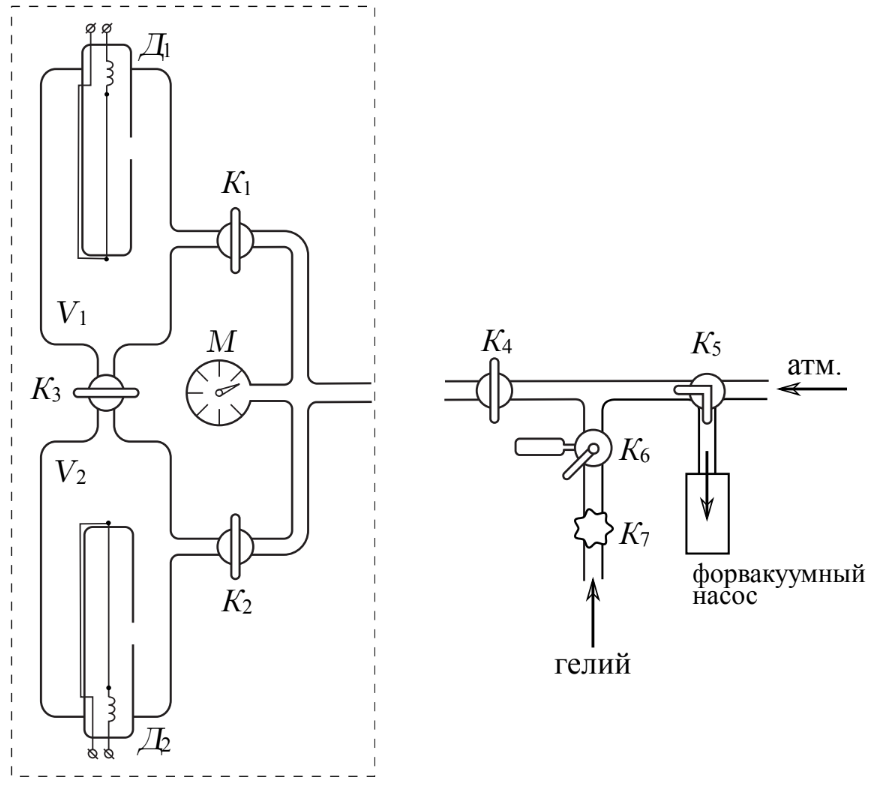
\includegraphics[scale=0.4]{physlabwork_6week_setup.png}\caption{Схема установки}\label{figure1}
\end{center}
\end{figure}
\begin{figure}%
    \centering
    \subfloat[\centering Двухходовый кран с дозатором]{{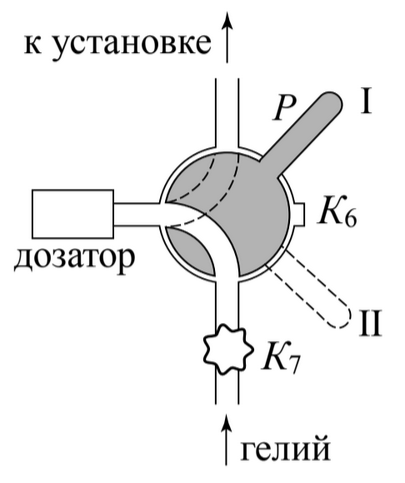
\includegraphics[width=5cm]{physlabwork_6week_setup_2.png} }}%
    \qquad
    \subfloat[\centering Мостовая электрическая схема]{{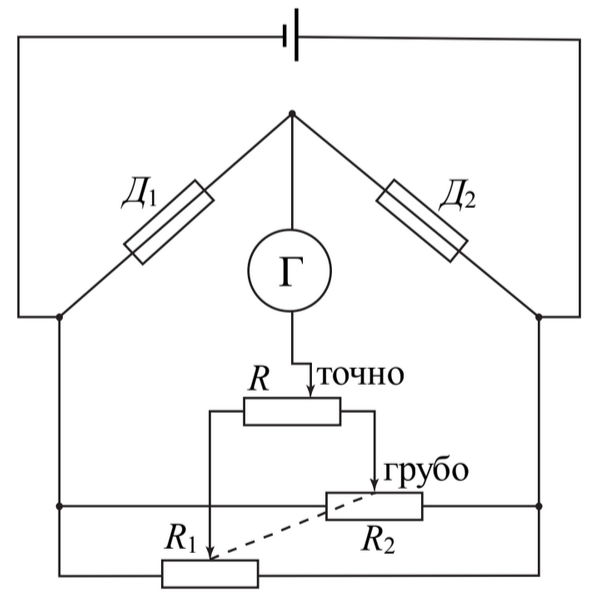
\includegraphics[width=5cm]{physlabwork_6week_setup_3.png} }}%
    \caption{Схемы дозатора и моста}%
    \label{}%
\end{figure}
\newpage
\section{Результаты измерений и обработка данных}
\includesvg[scale=0.7]{physlabwork_6week_37.svg}
\includesvg[scale=0.7]{physlabwork_6week_93.svg}
\includesvg[scale=0.7]{physlabwork_6week_141.svg}
\includesvg[scale=0.7]{physlabwork_6week_196.svg}
\includesvg[scale=0.7]{physlabwork_6week.svg}
\section{Обсуждение результатов}
\begin{equation*}
    D_{exp} = (6.32 \pm ) \cdot 10^{-5} \frac{m^2}{s}
\end{equation*}
\begin{equation*}
    D_{known} = (7.00 \pm ) \cdot 10^{-5} \frac{m^2}{s}
\end{equation*}
\section{Заключение}
В данной работе получена экспериментальная зависимость коэффициента взаимной диффузии от давления, которая в пределах погрешности совпадает с теорией. Также получен коэффициент взаимной диффузиии смеси воздух-гелий при нормальных условиях, который совпадает с табличным в пределах погрешности.
\end{document}
